\section{Hierarchical}
	Il clustering gerarchico è una delle tecniche di clustering popolari in quanto non richiede di sapere già il numero di clusters.
	\\[1\baselineskip]
	Si divide in due principali metodi di clustering:
		\begin{itemize}
			\item $\textbf{Agglomerativo}:$ utilizza una strategia $\textit{bottom-up}$:
				inizialmente ogni oggetto forma il proprio cluster, che viene unito iterativamente fino a quando un singolo cluster diventa la radice della gerarchia;

			\item $\textbf{Divisivo}:$ utilizza una strategia $\textit{top-down}$: 
				inizialmente tutti gli oggetti formano un singolo cluster, che viene ricorsivamente suddiviso in cluster più piccoli.
		\end{itemize}

	\clearpage

	\subsection{Algoritmo A.H.C.}
		$\textbf{Agglomerative Hierarchical Clustering}$ (A.H.C.) è un metodo di clustering il cui principio è semplice:
			\begin{enumerate}
				\item Il processo inizia calcolando la dissomiglianza tra gli $n$ oggetti;
				\item Due oggetti che, quando raggruppati insieme, minimizzano un dato criterio di agglomerazione, vengono raggruppati insieme creando così una classe che comprende questi due oggetti;
				\item Quindi la dissomiglianza tra questa classe e gli altri $n-2$ oggetti viene calcolata utilizzando il criterio di agglomerazione.
					\\
					I due oggetti o classi di oggetti il cui raggruppamento minimizza il criterio di agglomerazione vengono quindi raggruppati insieme.
			\end{enumerate}

			Questo processo continua finché tutti gli oggetti non sono stati raggruppati.
			\\[1\baselineskip]
			Queste operazioni di clustering producono un albero di clustering binario, chiamato $\textbf{dendrogramma}$, la cui radice è la classe che contiene tutte le osservazioni.
			Questo dendrogramma rappresenta una gerarchia di partizioni.
			È quindi possibile scegliere una partizione troncando l'albero a un dato livello, livello che dipende da vincoli definiti dall'utente (l'utente sa quante classi devono essere ottenute) o da criteri più oggettivi.

	\subsection{Algoritmo D.H.C.}
		$\textbf{Divisive Hierarchical Clustering}$ è un approccio di clustering in cui inizialmente tutti i punti nel dataset appartengono a un singolo cluster e la divisione viene eseguita in modo ricorsivo man mano che si scende nella gerarchia.
		\\[1\baselineskip]
		Gli steps che segue l'algoritmo sono:
			\begin{enumerate}
				\item Inizialmente, tutti i punti nel dataset appartengono a un singolo cluster;
				\item Partiziona il cluster in due cluster, il meno simili tra loro;
				\item Ad ogni iterazione, il cluster più eterogeneo viene diviso in due cluster;
				\item Procede con le iterazioni fino a che tutti gli oggetti sono nel loro cluster.
			\end{enumerate}
		
	\begin{figure}[h]
		\caption{Esempio di Clustering Agglomerativo e Divisivo}
		\centering
		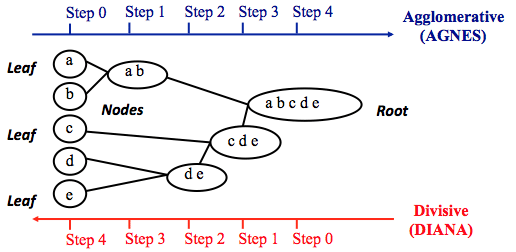
\includegraphics[width = 10cm]{AHC-DHC-examples.png}
	\end{figure}

\clearpage